% Created by tikzDevice version 0.12.4 on 2023-05-08 02:50:31
% !TEX encoding = UTF-8 Unicode
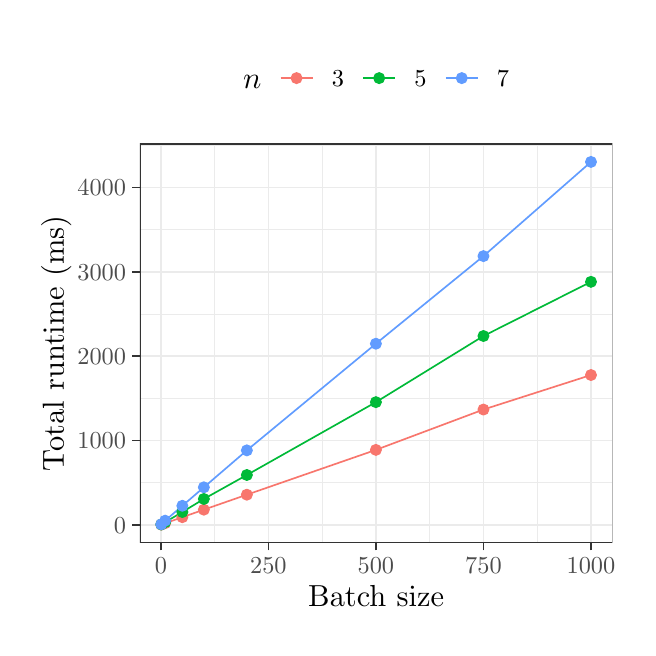
\begin{tikzpicture}[x=1pt,y=1pt]
\definecolor{fillColor}{RGB}{255,255,255}
\path[use as bounding box,fill=fillColor,fill opacity=0.00] (0,0) rectangle (216.81,216.81);
\begin{scope}
\path[clip] (  0.00,  0.00) rectangle (216.81,216.81);
\definecolor{drawColor}{RGB}{255,255,255}
\definecolor{fillColor}{RGB}{255,255,255}

\path[draw=drawColor,line width= 0.6pt,line join=round,line cap=round,fill=fillColor] (  0.00,  0.00) rectangle (216.81,216.81);
\end{scope}
\begin{scope}
\path[clip] ( 40.51, 30.69) rectangle (211.31,174.86);
\definecolor{fillColor}{RGB}{255,255,255}

\path[fill=fillColor] ( 40.51, 30.69) rectangle (211.31,174.86);
\definecolor{drawColor}{gray}{0.92}

\path[draw=drawColor,line width= 0.3pt,line join=round] ( 40.51, 52.41) --
	(211.31, 52.41);

\path[draw=drawColor,line width= 0.3pt,line join=round] ( 40.51, 82.89) --
	(211.31, 82.89);

\path[draw=drawColor,line width= 0.3pt,line join=round] ( 40.51,113.37) --
	(211.31,113.37);

\path[draw=drawColor,line width= 0.3pt,line join=round] ( 40.51,143.84) --
	(211.31,143.84);

\path[draw=drawColor,line width= 0.3pt,line join=round] ( 40.51,174.32) --
	(211.31,174.32);

\path[draw=drawColor,line width= 0.3pt,line join=round] ( 67.55, 30.69) --
	( 67.55,174.86);

\path[draw=drawColor,line width= 0.3pt,line join=round] (106.40, 30.69) --
	(106.40,174.86);

\path[draw=drawColor,line width= 0.3pt,line join=round] (145.26, 30.69) --
	(145.26,174.86);

\path[draw=drawColor,line width= 0.3pt,line join=round] (184.12, 30.69) --
	(184.12,174.86);

\path[draw=drawColor,line width= 0.6pt,line join=round] ( 40.51, 37.17) --
	(211.31, 37.17);

\path[draw=drawColor,line width= 0.6pt,line join=round] ( 40.51, 67.65) --
	(211.31, 67.65);

\path[draw=drawColor,line width= 0.6pt,line join=round] ( 40.51, 98.13) --
	(211.31, 98.13);

\path[draw=drawColor,line width= 0.6pt,line join=round] ( 40.51,128.60) --
	(211.31,128.60);

\path[draw=drawColor,line width= 0.6pt,line join=round] ( 40.51,159.08) --
	(211.31,159.08);

\path[draw=drawColor,line width= 0.6pt,line join=round] ( 48.12, 30.69) --
	( 48.12,174.86);

\path[draw=drawColor,line width= 0.6pt,line join=round] ( 86.98, 30.69) --
	( 86.98,174.86);

\path[draw=drawColor,line width= 0.6pt,line join=round] (125.83, 30.69) --
	(125.83,174.86);

\path[draw=drawColor,line width= 0.6pt,line join=round] (164.69, 30.69) --
	(164.69,174.86);

\path[draw=drawColor,line width= 0.6pt,line join=round] (203.55, 30.69) --
	(203.55,174.86);
\definecolor{drawColor}{RGB}{248,118,109}

\path[draw=drawColor,line width= 0.6pt,line join=round] ( 48.27, 37.24) --
	( 49.67, 37.74) --
	( 55.89, 39.92) --
	( 63.66, 42.64) --
	( 79.20, 48.05) --
	(125.83, 64.24) --
	(164.69, 78.82) --
	(203.55, 91.29);
\definecolor{drawColor}{RGB}{0,186,56}

\path[draw=drawColor,line width= 0.6pt,line join=round] ( 48.27, 37.28) --
	( 49.67, 38.11) --
	( 55.89, 41.79) --
	( 63.66, 46.51) --
	( 79.20, 55.17) --
	(125.83, 81.49) --
	(164.69,105.39) --
	(203.55,124.97);
\definecolor{drawColor}{RGB}{97,156,255}

\path[draw=drawColor,line width= 0.6pt,line join=round] ( 48.27, 37.35) --
	( 49.67, 38.66) --
	( 55.89, 44.04) --
	( 63.66, 50.72) --
	( 79.20, 64.07) --
	(125.83,102.61) --
	(164.69,134.26) --
	(203.55,168.30);
\definecolor{drawColor}{RGB}{248,118,109}
\definecolor{fillColor}{RGB}{248,118,109}

\path[draw=drawColor,line width= 0.4pt,line join=round,line cap=round,fill=fillColor] ( 48.27, 37.24) circle (  1.96);

\path[draw=drawColor,line width= 0.4pt,line join=round,line cap=round,fill=fillColor] ( 49.67, 37.74) circle (  1.96);

\path[draw=drawColor,line width= 0.4pt,line join=round,line cap=round,fill=fillColor] ( 63.66, 42.64) circle (  1.96);

\path[draw=drawColor,line width= 0.4pt,line join=round,line cap=round,fill=fillColor] (203.55, 91.29) circle (  1.96);

\path[draw=drawColor,line width= 0.4pt,line join=round,line cap=round,fill=fillColor] ( 79.20, 48.05) circle (  1.96);

\path[draw=drawColor,line width= 0.4pt,line join=round,line cap=round,fill=fillColor] ( 55.89, 39.92) circle (  1.96);

\path[draw=drawColor,line width= 0.4pt,line join=round,line cap=round,fill=fillColor] (125.83, 64.24) circle (  1.96);

\path[draw=drawColor,line width= 0.4pt,line join=round,line cap=round,fill=fillColor] (164.69, 78.82) circle (  1.96);
\definecolor{drawColor}{RGB}{0,186,56}
\definecolor{fillColor}{RGB}{0,186,56}

\path[draw=drawColor,line width= 0.4pt,line join=round,line cap=round,fill=fillColor] ( 48.27, 37.28) circle (  1.96);

\path[draw=drawColor,line width= 0.4pt,line join=round,line cap=round,fill=fillColor] ( 49.67, 38.11) circle (  1.96);

\path[draw=drawColor,line width= 0.4pt,line join=round,line cap=round,fill=fillColor] ( 63.66, 46.51) circle (  1.96);

\path[draw=drawColor,line width= 0.4pt,line join=round,line cap=round,fill=fillColor] (203.55,124.97) circle (  1.96);

\path[draw=drawColor,line width= 0.4pt,line join=round,line cap=round,fill=fillColor] ( 79.20, 55.17) circle (  1.96);

\path[draw=drawColor,line width= 0.4pt,line join=round,line cap=round,fill=fillColor] ( 55.89, 41.79) circle (  1.96);

\path[draw=drawColor,line width= 0.4pt,line join=round,line cap=round,fill=fillColor] (125.83, 81.49) circle (  1.96);

\path[draw=drawColor,line width= 0.4pt,line join=round,line cap=round,fill=fillColor] (164.69,105.39) circle (  1.96);
\definecolor{drawColor}{RGB}{97,156,255}
\definecolor{fillColor}{RGB}{97,156,255}

\path[draw=drawColor,line width= 0.4pt,line join=round,line cap=round,fill=fillColor] ( 48.27, 37.35) circle (  1.96);

\path[draw=drawColor,line width= 0.4pt,line join=round,line cap=round,fill=fillColor] ( 49.67, 38.66) circle (  1.96);

\path[draw=drawColor,line width= 0.4pt,line join=round,line cap=round,fill=fillColor] ( 63.66, 50.72) circle (  1.96);

\path[draw=drawColor,line width= 0.4pt,line join=round,line cap=round,fill=fillColor] (203.55,168.30) circle (  1.96);

\path[draw=drawColor,line width= 0.4pt,line join=round,line cap=round,fill=fillColor] ( 79.20, 64.07) circle (  1.96);

\path[draw=drawColor,line width= 0.4pt,line join=round,line cap=round,fill=fillColor] ( 55.89, 44.04) circle (  1.96);

\path[draw=drawColor,line width= 0.4pt,line join=round,line cap=round,fill=fillColor] (125.83,102.61) circle (  1.96);

\path[draw=drawColor,line width= 0.4pt,line join=round,line cap=round,fill=fillColor] (164.69,134.26) circle (  1.96);
\definecolor{drawColor}{gray}{0.20}

\path[draw=drawColor,line width= 0.6pt,line join=round,line cap=round] ( 40.51, 30.69) rectangle (211.31,174.86);
\end{scope}
\begin{scope}
\path[clip] (  0.00,  0.00) rectangle (216.81,216.81);
\definecolor{drawColor}{gray}{0.30}

\node[text=drawColor,anchor=base east,inner sep=0pt, outer sep=0pt, scale=  0.88] at ( 35.56, 34.14) {0};

\node[text=drawColor,anchor=base east,inner sep=0pt, outer sep=0pt, scale=  0.88] at ( 35.56, 64.62) {1000};

\node[text=drawColor,anchor=base east,inner sep=0pt, outer sep=0pt, scale=  0.88] at ( 35.56, 95.10) {2000};

\node[text=drawColor,anchor=base east,inner sep=0pt, outer sep=0pt, scale=  0.88] at ( 35.56,125.57) {3000};

\node[text=drawColor,anchor=base east,inner sep=0pt, outer sep=0pt, scale=  0.88] at ( 35.56,156.05) {4000};
\end{scope}
\begin{scope}
\path[clip] (  0.00,  0.00) rectangle (216.81,216.81);
\definecolor{drawColor}{gray}{0.20}

\path[draw=drawColor,line width= 0.6pt,line join=round] ( 37.76, 37.17) --
	( 40.51, 37.17);

\path[draw=drawColor,line width= 0.6pt,line join=round] ( 37.76, 67.65) --
	( 40.51, 67.65);

\path[draw=drawColor,line width= 0.6pt,line join=round] ( 37.76, 98.13) --
	( 40.51, 98.13);

\path[draw=drawColor,line width= 0.6pt,line join=round] ( 37.76,128.60) --
	( 40.51,128.60);

\path[draw=drawColor,line width= 0.6pt,line join=round] ( 37.76,159.08) --
	( 40.51,159.08);
\end{scope}
\begin{scope}
\path[clip] (  0.00,  0.00) rectangle (216.81,216.81);
\definecolor{drawColor}{gray}{0.20}

\path[draw=drawColor,line width= 0.6pt,line join=round] ( 48.12, 27.94) --
	( 48.12, 30.69);

\path[draw=drawColor,line width= 0.6pt,line join=round] ( 86.98, 27.94) --
	( 86.98, 30.69);

\path[draw=drawColor,line width= 0.6pt,line join=round] (125.83, 27.94) --
	(125.83, 30.69);

\path[draw=drawColor,line width= 0.6pt,line join=round] (164.69, 27.94) --
	(164.69, 30.69);

\path[draw=drawColor,line width= 0.6pt,line join=round] (203.55, 27.94) --
	(203.55, 30.69);
\end{scope}
\begin{scope}
\path[clip] (  0.00,  0.00) rectangle (216.81,216.81);
\definecolor{drawColor}{gray}{0.30}

\node[text=drawColor,anchor=base,inner sep=0pt, outer sep=0pt, scale=  0.88] at ( 48.12, 19.68) {0};

\node[text=drawColor,anchor=base,inner sep=0pt, outer sep=0pt, scale=  0.88] at ( 86.98, 19.68) {250};

\node[text=drawColor,anchor=base,inner sep=0pt, outer sep=0pt, scale=  0.88] at (125.83, 19.68) {500};

\node[text=drawColor,anchor=base,inner sep=0pt, outer sep=0pt, scale=  0.88] at (164.69, 19.68) {750};

\node[text=drawColor,anchor=base,inner sep=0pt, outer sep=0pt, scale=  0.88] at (203.55, 19.68) {1000};
\end{scope}
\begin{scope}
\path[clip] (  0.00,  0.00) rectangle (216.81,216.81);
\definecolor{drawColor}{RGB}{0,0,0}

\node[text=drawColor,anchor=base,inner sep=0pt, outer sep=0pt, scale=  1.10] at (125.91,  7.64) {Batch size};
\end{scope}
\begin{scope}
\path[clip] (  0.00,  0.00) rectangle (216.81,216.81);
\definecolor{drawColor}{RGB}{0,0,0}

\node[text=drawColor,rotate= 90.00,anchor=base,inner sep=0pt, outer sep=0pt, scale=  1.10] at ( 13.08,102.77) {Total runtime (ms)};
\end{scope}
\begin{scope}
\path[clip] (  0.00,  0.00) rectangle (216.81,216.81);
\definecolor{fillColor}{RGB}{255,255,255}

\path[fill=fillColor] ( 72.33,185.86) rectangle (179.49,211.31);
\end{scope}
\begin{scope}
\path[clip] (  0.00,  0.00) rectangle (216.81,216.81);
\definecolor{drawColor}{RGB}{0,0,0}

\node[text=drawColor,anchor=base west,inner sep=0pt, outer sep=0pt, scale=  1.10] at ( 77.83,194.80) {$n$};
\end{scope}
\begin{scope}
\path[clip] (  0.00,  0.00) rectangle (216.81,216.81);
\definecolor{fillColor}{RGB}{255,255,255}

\path[fill=fillColor] ( 89.93,191.36) rectangle (104.39,205.81);
\end{scope}
\begin{scope}
\path[clip] (  0.00,  0.00) rectangle (216.81,216.81);
\definecolor{drawColor}{RGB}{248,118,109}

\path[draw=drawColor,line width= 0.6pt,line join=round] ( 91.38,198.58) -- (102.94,198.58);
\end{scope}
\begin{scope}
\path[clip] (  0.00,  0.00) rectangle (216.81,216.81);
\definecolor{drawColor}{RGB}{248,118,109}
\definecolor{fillColor}{RGB}{248,118,109}

\path[draw=drawColor,line width= 0.4pt,line join=round,line cap=round,fill=fillColor] ( 97.16,198.58) circle (  1.96);
\end{scope}
\begin{scope}
\path[clip] (  0.00,  0.00) rectangle (216.81,216.81);
\definecolor{fillColor}{RGB}{255,255,255}

\path[fill=fillColor] (119.78,191.36) rectangle (134.24,205.81);
\end{scope}
\begin{scope}
\path[clip] (  0.00,  0.00) rectangle (216.81,216.81);
\definecolor{drawColor}{RGB}{0,186,56}

\path[draw=drawColor,line width= 0.6pt,line join=round] (121.23,198.58) -- (132.79,198.58);
\end{scope}
\begin{scope}
\path[clip] (  0.00,  0.00) rectangle (216.81,216.81);
\definecolor{drawColor}{RGB}{0,186,56}
\definecolor{fillColor}{RGB}{0,186,56}

\path[draw=drawColor,line width= 0.4pt,line join=round,line cap=round,fill=fillColor] (127.01,198.58) circle (  1.96);
\end{scope}
\begin{scope}
\path[clip] (  0.00,  0.00) rectangle (216.81,216.81);
\definecolor{fillColor}{RGB}{255,255,255}

\path[fill=fillColor] (149.64,191.36) rectangle (164.09,205.81);
\end{scope}
\begin{scope}
\path[clip] (  0.00,  0.00) rectangle (216.81,216.81);
\definecolor{drawColor}{RGB}{97,156,255}

\path[draw=drawColor,line width= 0.6pt,line join=round] (151.08,198.58) -- (162.65,198.58);
\end{scope}
\begin{scope}
\path[clip] (  0.00,  0.00) rectangle (216.81,216.81);
\definecolor{drawColor}{RGB}{97,156,255}
\definecolor{fillColor}{RGB}{97,156,255}

\path[draw=drawColor,line width= 0.4pt,line join=round,line cap=round,fill=fillColor] (156.86,198.58) circle (  1.96);
\end{scope}
\begin{scope}
\path[clip] (  0.00,  0.00) rectangle (216.81,216.81);
\definecolor{drawColor}{RGB}{0,0,0}

\node[text=drawColor,anchor=base west,inner sep=0pt, outer sep=0pt, scale=  0.88] at (109.89,195.55) {3};
\end{scope}
\begin{scope}
\path[clip] (  0.00,  0.00) rectangle (216.81,216.81);
\definecolor{drawColor}{RGB}{0,0,0}

\node[text=drawColor,anchor=base west,inner sep=0pt, outer sep=0pt, scale=  0.88] at (139.74,195.55) {5};
\end{scope}
\begin{scope}
\path[clip] (  0.00,  0.00) rectangle (216.81,216.81);
\definecolor{drawColor}{RGB}{0,0,0}

\node[text=drawColor,anchor=base west,inner sep=0pt, outer sep=0pt, scale=  0.88] at (169.59,195.55) {7};
\end{scope}
\end{tikzpicture}
